\documentclass{beamer}
%
% Choose how your presentation looks.
%
% For more themes, color themes and font themes, see:
% http://deic.uab.es/~iblanes/beamer_gallery/index_by_theme.html
%
\mode<presentation>
{
  \usetheme{default}      % or try Darmstadt, Madrid, Warsaw, ...
  \usecolortheme{default} % or try albatross, beaver, crane, ...
  \usefonttheme{default}  % or try serif, structurebold, ...
  \setbeamertemplate{navigation symbols}{}
  \setbeamertemplate{caption}[numbered]
} 
\usepackage{amsmath}

\DeclareMathOperator{\taninv}{tan\,inverse}

\usepackage[english]{babel}
\usepackage{physics}
\usepackage[utf8]{inputenc}
\usepackage[T1]{fontenc}

\title[Your Short Title]{Gate problem}
\author{Kuntal Kokate}

\institute{EE18BTECH11028}
\date{\today}

\begin{document}

\begin{frame}
  \titlepage
\end{frame}

% Uncomment these lines for an automatically generated outline.
%\begin{frame}{Outline}
%  \tableofcontents
%\end{frame}

\section{Introduction}

\begin{frame}{Problem statement}

\begin{itemize}
  \item EC 2017 Q.34
  
\end{itemize}

\vskip 1cm

\begin{block}{Problem}
The transfer function of causal L.T.I system is $ H(s) = \frac{1}{s}$. If the input to the system is 
$x(t) = (\frac{sin(t)}{\pi*t})u(t)$, where u(t) is a unit step function, the system output 
$y(t)$ as $t \to \infty$  is ?
\end{block}

\end{frame}

\section{Some \LaTeX{} Examples}

\subsection{Solution}
\begin{frame}{Solution}
let $f(t) = sin(t)u(t)$
\newline
We know that, $\mathcal{L}\{f(t)\} = F(s) = \frac{1}{1 + s^2} $
    ( u.v rule of integration.)
\newline
By using,  $\mathcal{L}\{\frac{f(t)}{t}\} = \int_{s}^{\infty}F(s) \dd{s} $
\newline
\newline
$\implies$ $X(s) = (1/ \pi)( \frac{\pi}{2} - \taninv(s))$
\newline
\newline
$\implies$ $Y(s) = (1/ \pi s) ( \frac{\pi}{2} - \taninv(s))$ , (since $Y(s) = X(s)H(s)$)
\newline
\newline
\[y(\infty) = \lim_{s\to\ 0} sY(s) =(\frac{1}{\pi}) ( \frac{\pi}{2} - \taninv(s)) = \frac{1}{2}\]
\hspace{1cm} (Using Final value theorem.)

\end{frame}

\begin{frame}{Proof of Final Value Theorem: }
The last statement is implied by final value theorem.
\newline
\newline
To prove: $\lim_{s\to\ 0} (s*F(s)) = \lim_{t\to\infty} f(t)$
\newline
\newline
Proof:
\newline
\newline
We know, 
$\mathcal{L}\{\pdv{f(t)}{t}\} = \int_{0^-}^{\infty} \pdv{f(t)}{t} e^{-st}\dd{t} =s*F(s)-f(0^{-}) $
\newline
\newline
Now applying $ s \to 0$, \hfill
\newline
\newline
We have,  RHS $=\int_{0^-}^{\infty} \pdv{f}{t}\dd{t} = \lim_{s\to\ 0}(f(\infty) - f(0^{-})) $
\newline
\newline
And ,  $LHS$ $= \lim_{s\to\ 0}(s.F(s)-f(0^{-}))$
\newline
Hence proved


\end{frame}

\begin{frame}{Verification}
\begin{figure}[h]
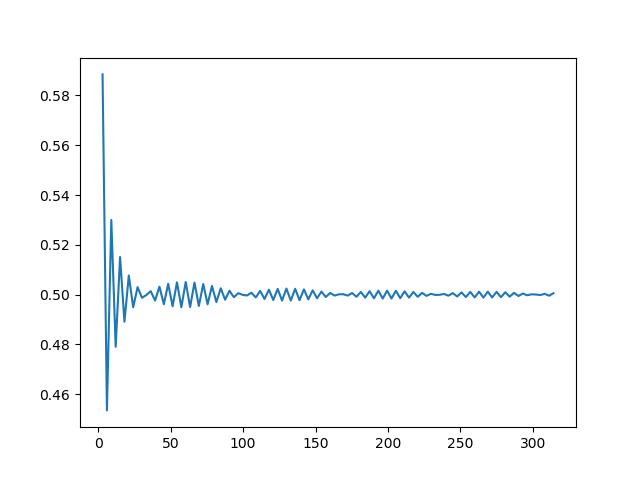
\includegraphics[width=8cm]{verification.png}
\end{figure}

    
\end{frame}



\end{document}
